\documentclass[tikz]{standalone}
\usepackage{tikz}


\begin{document}    
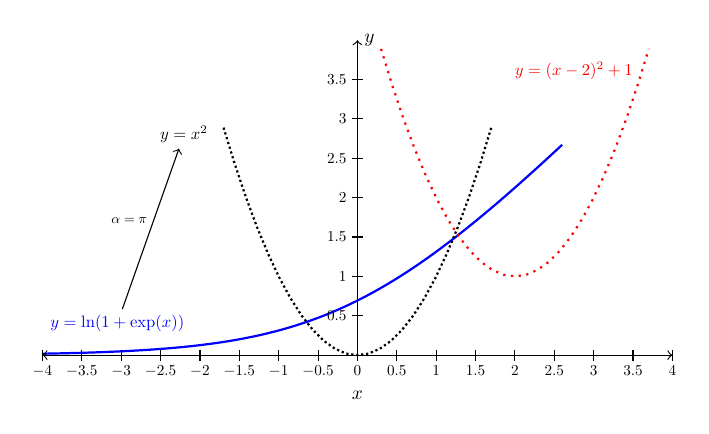
\begin{tikzpicture}
 \usetikzlibrary{positioning}
 
% center of the graph 
\node (center) {};
 

%Functions to be plotted
\draw[scale=1, domain=-4:2.6, smooth ,variable=\x, blue,thick] plot  ({\x}, {ln(1+exp(\x))});
\draw[scale=1, domain=0.3:3.7,  dotted ,variable=\x, red,thick] plot  ({\x}, {(\x-2)*(\x-2)+ 1}   );
\draw[scale=1, domain=-1.7:1.7, densely dotted ,variable=\x, black,thick] plot  ({\x}, {\x*\x});

 %Name
\node (quadratic1) [scale=0.6,above right=3.3cm and 1.8cm of center,red ] {$y=(x-2)^{2} + 1$};
\node (quadratic2) [scale=0.6,above left=2.5cm and 1.7cm of center,black ] {$y=x^{2}$};
\node (logsum) [scale=0.6,above left=0.1cm and 2cm of center,blue ] {$y=\ln(1 + \exp(x))$};

  
%Axis
\draw[<->] (-4, 0) -- (4, 0) node[scale=0.7,below left= 0.25cm and -.28cm of center] {$x$};
\draw[->] (0,0 ) -- (0, 4) node[right,scale=0.7] {$y$};

%Draw Axis numbers by hand using a loop
\foreach \x/\xtext in {0,0.5,1,1.5,2,2.5,3,3.5,4}
\draw[shift={(\x,0)}] (0pt,2pt) -- (0pt,-2pt) node[scale=0.55,below] {$\xtext$};

\foreach \x/\xtext in {0.5,1,1.5,2,2.5,3,3.5,4}
\draw[shift={(-\x,0)}] (0pt,2pt) -- (0pt,-2pt) node[scale=0.55,below] {$-\xtext$};

\foreach \y/\ytext in {0.5,1,1.5,2,2.5,3,3.5}
\draw[shift={(0,\y)}] (2pt,0pt) -- (-2pt,0pt) node[scale=0.55,left] {$\ytext$};
  

%Draw lines with messages using nodes
\draw [->] (logsum) -- node[name=yes,above,text width=2cm,midway,scale=0.5]  {$\alpha=\pi$} (quadratic2);



  
\end{tikzpicture}
\end{document}


